\section{Sequential structures}
\only<article>{The simplest type of structure in data is sequences. Examples include speech, text and DNA sequences, as well as data acquired in any sequential decision making problem such as recommendation systems or robotics. Sequential data is always thought to arise from some Markovian processes, defined below.}

\only<presentation>{
  \begin{frame}
    \centering
    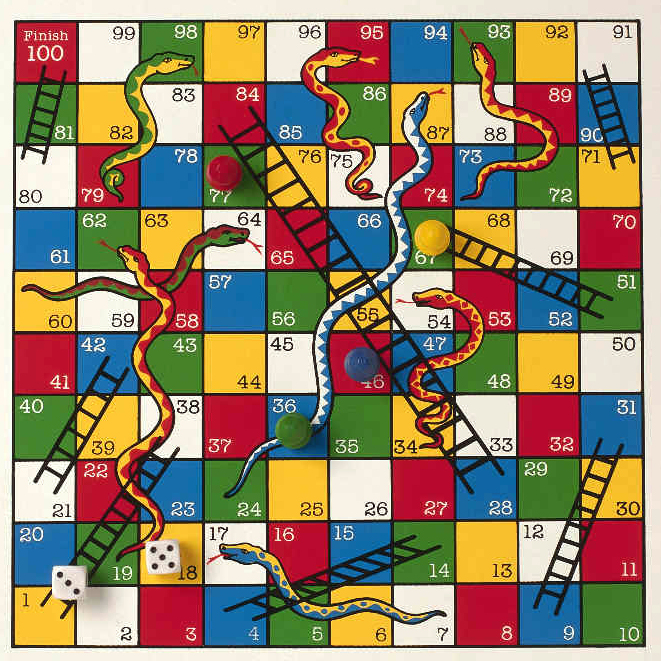
\includegraphics[height=\textheight]{../figures/Snake-And-Ladder}
  \end{frame}
}
\begin{frame}
\frametitle{Markov process}
  \begin{figure}[H]
    \centering
    \begin{tikzpicture}
      \node[RV] at (-2,0) (xt1) {$x_{t-1}$};
      \node[RV] at (0,0) (xt2) {$x_t$};
      \node[RV] at (2,0) (xt3) {$x_{t+1}$};
      \draw[->] (xt1)--(xt2);
      \draw[->] (xt2)--(xt3);
    \end{tikzpicture}
    \label{fig:markov-chain}
    \caption{Graphical model for a Markov process.}
  \end{figure}
  \begin{definition}[Markov process]
    A Markov process is a sequence of variables $x_t : \Omega \to \CX$ such that $x_{t+1} \mid x_t \indep x_{t-k} \forall k \leq 1$.
  \end{definition}
  \begin{block}{Application}
    \begin{itemize}
    \item Sequence compression (especially with variable order Models).
    \item Web-search (Page-Rank)
    \item Hidden Markov Models.
    \item MCMC.
    \end{itemize}
  \end{block}

\end{frame}



\begin{frame}
\frametitle{Hidden Markov model}
\only<article>{Frequently the sequential dependency is not in the data itself, but in some hidden underlying markov process. In that case, the hidden variable $x_t$ is the \emph{state} of the process. The observed variable $y_t$ is simply an observation.}
  \begin{figure}[H]
    \centering
    \begin{tikzpicture}
      \node[RV, hidden] at (-2,0) (xt1) {$x_{t-1}$};
      \node[RV, hidden] at (0,0) (xt2) {$x_t$};
      \node[RV, hidden] at (2,0) (xt3) {$x_{t+1}$};
      \node[RV] at (-2,2) (yt1) {$y_{t-1}$};
      \node[RV] at (0,2) (yt2) {$y_t$};
      \node[RV] at (2,2) (yt3) {$y_{t+1}$};
      \draw[->] (xt1)--(xt2);
      \draw[->] (xt2)--(xt3);
      \draw[->] (xt1)--(yt1);
      \draw[->] (xt2)--(yt2);
      \draw[->] (xt3)--(yt3);
    \end{tikzpicture}
    \label{fig:markov-chain}
    \caption{Graphical model for a hidden Markov model.}
  \end{figure}
  \begin{align}
    \label{eq:hmm}
    P_\param(x_{t+1} \mid x_t) \tag{transition distribution}\\
    P_\param(y_t \mid x_t) \tag{emission distribution}
  \end{align}
  \only<article>{For any given parater value $\param$, it is easy to estimate the probability distribution over states given the observations $P_\param(x^T \mid y^T)$. As an example, if $y^T$ is raw speech data and $x^T$ is a sequence of words, and $\theta$ are the parameters of our speech model, then we can obtain probabilities for every possible sequence of words that was uttered. Frequently, though, in speech recognition we are only interested in the most likely seuence of words. This makes the problem simple enough to be solved instantaneously by modern cellphones.}
  \begin{block}{Application}
    \begin{itemize}
    \item Speech recognition.
    \item Filtering (Kalman Filter).
    \item DNA analysis.
    \end{itemize}
  \end{block}
\end{frame}




%%% Local Variables:
%%% mode: latex
%%% TeX-engine: xetex
%%% TeX-master: "notes.tex"
%%% End:
